% Figure 1.3 — The mismatch condition M(S) = L_actual △ L_σ
% For V4 §1.4. Shows Bridge #108 dissociation as symmetric difference of inhabited and self-described levels.
% Requires: tikz

\begin{figure}[htbp]
\centering
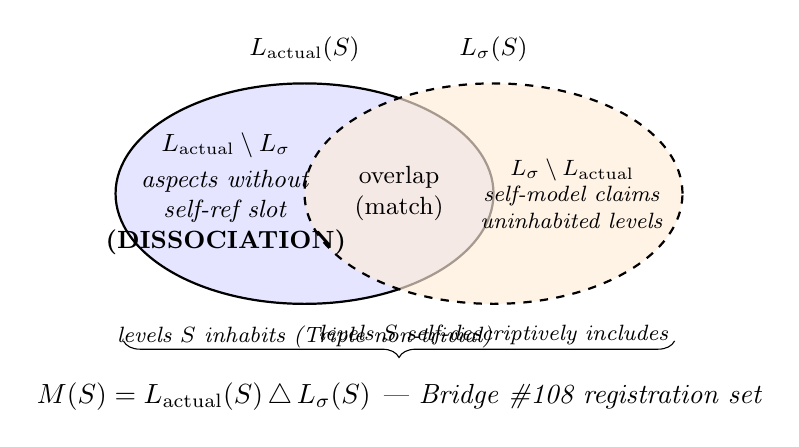
\begin{tikzpicture}[scale=1.0, every node/.style={font=\small}]
  % L_actual set (solid border)
  \draw[thick, fill=blue!10] (-1.2,0) ellipse (2.4 and 1.4);
  \node[above] at (-1.2, 1.55) {$L_{\mathrm{actual}}(S)$};
  \node[below, font=\footnotesize\itshape] at (-1.2, -1.55) {levels $S$ inhabits (Triple non-trivial)};

  % L_sigma set (dashed border)
  \draw[thick, dashed, fill=orange!15, fill opacity=0.65] (1.2,0) ellipse (2.4 and 1.4);
  \node[above] at (1.2, 1.55) {$L_{\sigma}(S)$};
  \node[below, font=\footnotesize\itshape] at (1.2, -1.55) {levels $S$ self-descriptively includes};

  % Labels inside
  \node at (-2.2, 0) [align=center, font=\small]
    {$L_{\mathrm{actual}} \setminus L_\sigma$\\[2pt]\textit{aspects without}\\\textit{self-ref slot}\\\textbf{(DISSOCIATION)}};
  \node at (0, 0) [align=center, font=\small] {overlap\\(match)};
  \node at (2.2, 0) [align=center, font=\footnotesize]
    {$L_\sigma \setminus L_{\mathrm{actual}}$\\\textit{self-model claims}\\\textit{uninhabited levels}};

  % M(S) bracket
  \draw [decorate, decoration={brace, amplitude=6pt, mirror, raise=2pt}]
    (-3.5, -1.8) -- (3.5, -1.8)
    node [midway, yshift=-22pt, font=\itshape]
    {$M(S) = L_{\mathrm{actual}}(S) \,\triangle\, L_\sigma(S)$ — Bridge~\#108 registration set};
\end{tikzpicture}
\caption{The mismatch condition. $L_{\mathrm{actual}}(S)$ is the set of carrier-levels at which $S$'s Triple is non-trivial (all three factors well-defined). $L_\sigma(S)$ is the set of levels $S$'s self-definition functor $\sigma_S$ picks out. The symmetric difference $M(S) = L_{\mathrm{actual}}(S) \triangle L_\sigma(S)$ is the registration set for Bridge \#108 dissociation: at levels in $L_{\mathrm{actual}} \setminus L_\sigma$, aspects of $X$ entangled with $\mathrm{K}_{L_i}(S)$ register in $S$'s experience without $\sigma_S$-slots to hold them. The multiplex-default corollary is the observation that, for $|L_{\mathrm{actual}}(S)| > 1$, mono-carrier self-models $|L_\sigma(S)| = 1$ guarantee $M(S) \neq \varnothing$. Integration is the operation $\sigma_S \mapsto \sigma_S'$ with $L_{\sigma'}(S) = L_{\mathrm{actual}}(S)$.}
\label{fig:mismatch-condition}
\end{figure}
